\chapter{Introduction}
Large Language Models (LLMs) have achieved remarkable capabilities across a range of tasks, from natural language understanding to complex reasoning. However, this prowess comes with steep resource demands that pose significant challenges for both training and deployment.

The exponential growth in large language model parameter counts and context lengths has created unprecedented computational and memory demands. State-of-the-art models often consist of billions of parameters, requiring substantial memory and computational power for training and inference. Traditional mixed-precision approaches using FP16 and BF16 formats, while effective, still impose significant memory overhead that limits model scalability and training throughput. For instance, training a 3 billion parameter model with BF16 precision requires over 82 GB of GPU memory, while an 8 billion parameter model demands similar or higher memory allocation.

The introduction of 8-bit floating-point (FP8) formats offers the potential to halve memory requirements while maintaining numerical stability, but current implementations face challenges in optimally leveraging the distinct characteristics of available FP8 variants. NVIDIA's standardization of two FP8 formats—E4M3 (4-bit exponent, 3-bit mantissa) and E5M2 (5-bit exponent, 2-bit mantissa)—presents a fundamental trade-off between precision and dynamic range. Existing FP8 training approaches predominantly employ uniform format assignment strategies, but our analysis reveals that different transformer components exhibit distinct computational patterns that benefit from different FP8 formats.

% \section{Problem}

\textbf{Low-bit quantization} has emerged as a promising solution to shrink model size and speed up computation, making deployment of LLMs on edge hardware more practical. Quantization involves using reduced numerical precision to represent model weights and activations. By compressing model parameters from the standard 32-bit floating point (FP32) down to 8-bit or lower, we can dramatically cut memory usage and computational load. Recent advances in mixed-precision techniques even allow combining different precisions (e.g. 16-bit and 4-bit) in one matrix multiplication operation to balance speed and accuracy. Hardware vendors and researchers are actively exploring ultra-low precision arithmetic (int8, int4, even binary) to push LLMs onto resource-constrained environments.
\section{Motivation}\label{sec:motivation}

Why are LLMs hard to deploy on edge devices? The fundamental issue is scale. Modern Transformer-based LLMs achieve higher accuracy primarily by scaling up parameter counts and training data. This leads to massive models that strain memory and compute resources. In general, deploying an LLM requires loading all its weights into memory (GPU VRAM or RAM) and performing billions of math operations per inference. Edge devices, however, are constrained in memory (often a few GB) and lack the specialized matrix acceleration of large data-center GPUs.

\subsection{Qwen2.5-1.5B and Efficient Small-Scale LLMs}
Powerful open-source models such as \textbf{Qwen 2.5} deliver impressive general-purpose performance, yet their accuracy deteriorates once the task domain narrows to highly structured mathematics.  Bridging that gap ordinarily requires full-parameter fine-tuning, a process that is both memory-hungry and compute-intensive for billion-parameter networks.  As a result, research laboratories and edge-computing practitioners alike face prohibitive costs when attempting to adapt state-of-the-art language models to specialized workloads.

Our objective is therefore two-fold: \emph{(i)} preserve the strong reasoning capabilities of Qwen 2.5 on domain-specific maths tasks, and \emph{(ii)} compress the computational footprint so the refined model can run on modest hardware budgets.  Recent accelerator generations provide two complementary avenues for achieving this goal.

\textbf{FP8 training.}  
NVIDIA Hopper- and AMD CDNA3-class GPUs expose native 8-bit floating-point (FP8) tensor cores.  Training directly in FP8 slashes memory consumption by up to 75 \% relative to FP32 while simultaneously boosting arithmetic throughput, enabling us to iterate on large models without resorting to multi-node clusters.

\textbf{FP8 post-training quantization.}  
Once fine-tuning converges, we further compress the model by converting all weight tensors from FP16/BF16 to FP8.  This step multiplies the capacity of a given GPU by roughly two, shortens inference latency, and lowers energy draw—without incurring a noticeable loss in perplexity or downstream accuracy.

By combining FP8-aware optimization with post-training quantization, the project demonstrates that \textsc{Qwen 2.5-1.5B} can retain its mathematical reasoning prowess while fitting within the memory envelope of a single H100 NVL or even smaller edge devices, thereby widening access to high-quality, domain-tuned language models.


\section{Dataset}
To train our reasoning model, we compiled a dataset covering many mathematical and logical problems. This dataset includes various problem types such as arithmetic operations, algebraic equations, logical reasoning, and multi-step problem solving to ensure comprehensive coverage of mathematical reasoning capabilities.
\section{Our Approach}\label{sec:approach}

Figure~\ref{fig:overview} provides an overview of the whole pipeline that we employ to create an effective mathematics-aware language model. Now the diagram is focused on the \textsc{Qwen2.5-1.5B} checkpoint, and this process can generalize to any decoder-only transformer of similar size. The pipeline consists of four successive stages, see below.\\

\textbf{(1) Data curation and pre-processing.}
We start by collecting various mathematics corpora: open-source proof repositories, competition problems, and questions which are selected from educational websites, question-answer pairs (QAPs). After removing duplicates, the raw pool has 3M candidate sentences. A lightweight heuristic filter discards non-mathematical text and malformed \LaTeX\ text, resulting in over 260 K high-quality examples. The token for each sample is then tokenized using the original \texttt{qwen.tiktoken} tokenizer and trimmed or zero-padded to a maximum length of 512 tokens to be compatible with the model’s context window.\\

\textbf{(2) Preparing the model.}
The vanilla Hugging Face checkpoint contains \texttt{nn.Linear}, \texttt{nn.LayerNorm}, and \texttt{RMSNorm} modules. We write a one-for-one replacement that exchanges these layers for their highest quality NVIDIA Transformer Engine (TE) counterpart, thus enabling native FP8 execution on Hopper GPUs without modifying the weight tensors. A configuration file also switches on grouped-query attention (GQA) and rotary positional embeddings so that the fine-tuned model follows the most recent Qwen2 architectural specifications.\\

\textbf{(3) Precision-Aware Fine-Tuning.}
We continue training for three epochs with a global batch size of 26 × 4 = 104 sequences, which we achieve using the gradient-accumulation loop from Section~\ref{sec:gradacc}. We adopt the hybrid FP8 recipe (E4M3 for weight/activations, E5M2 for gradients) explained in Section~\ref{sec:precision_recipes}. The learning-rate dynamics are controlled by an AdamW optimizer with \(\beta_1=0.9\), \(\beta_2=0.95\), and a 50 step cosine warm-up. Checkpoints are saved every 1,000 optimization steps along with parameter-efficient \texttt{wandb} logs of perplexity and token-level accuracy.\\

\textbf{(4) Serving/receiving and judging.}
At the end, the highest scoring FP8 checkpoint is transferred to the \texttt{vLLM} inference engine, which flows tokens with paged attention and speculative decoding. On a H100 NVL, during inference, we obtain a throughput of 102.5 tokens/s at a latency of 11.8 ms ± 0:2 ms using only 1:70 GiB of device memory. Functional correctness is tested against GSM8K and MATH dev sets, the fine-tuned model outperforms FP32 baseline in avg-exact-k by 4.6\% abs-pnt. The released final artifacts, i.e., the model weight, tokenizer, and evaluation scripts are licensed to be open to downstream research community.

    
\begin{figure}[h]
    \centering
    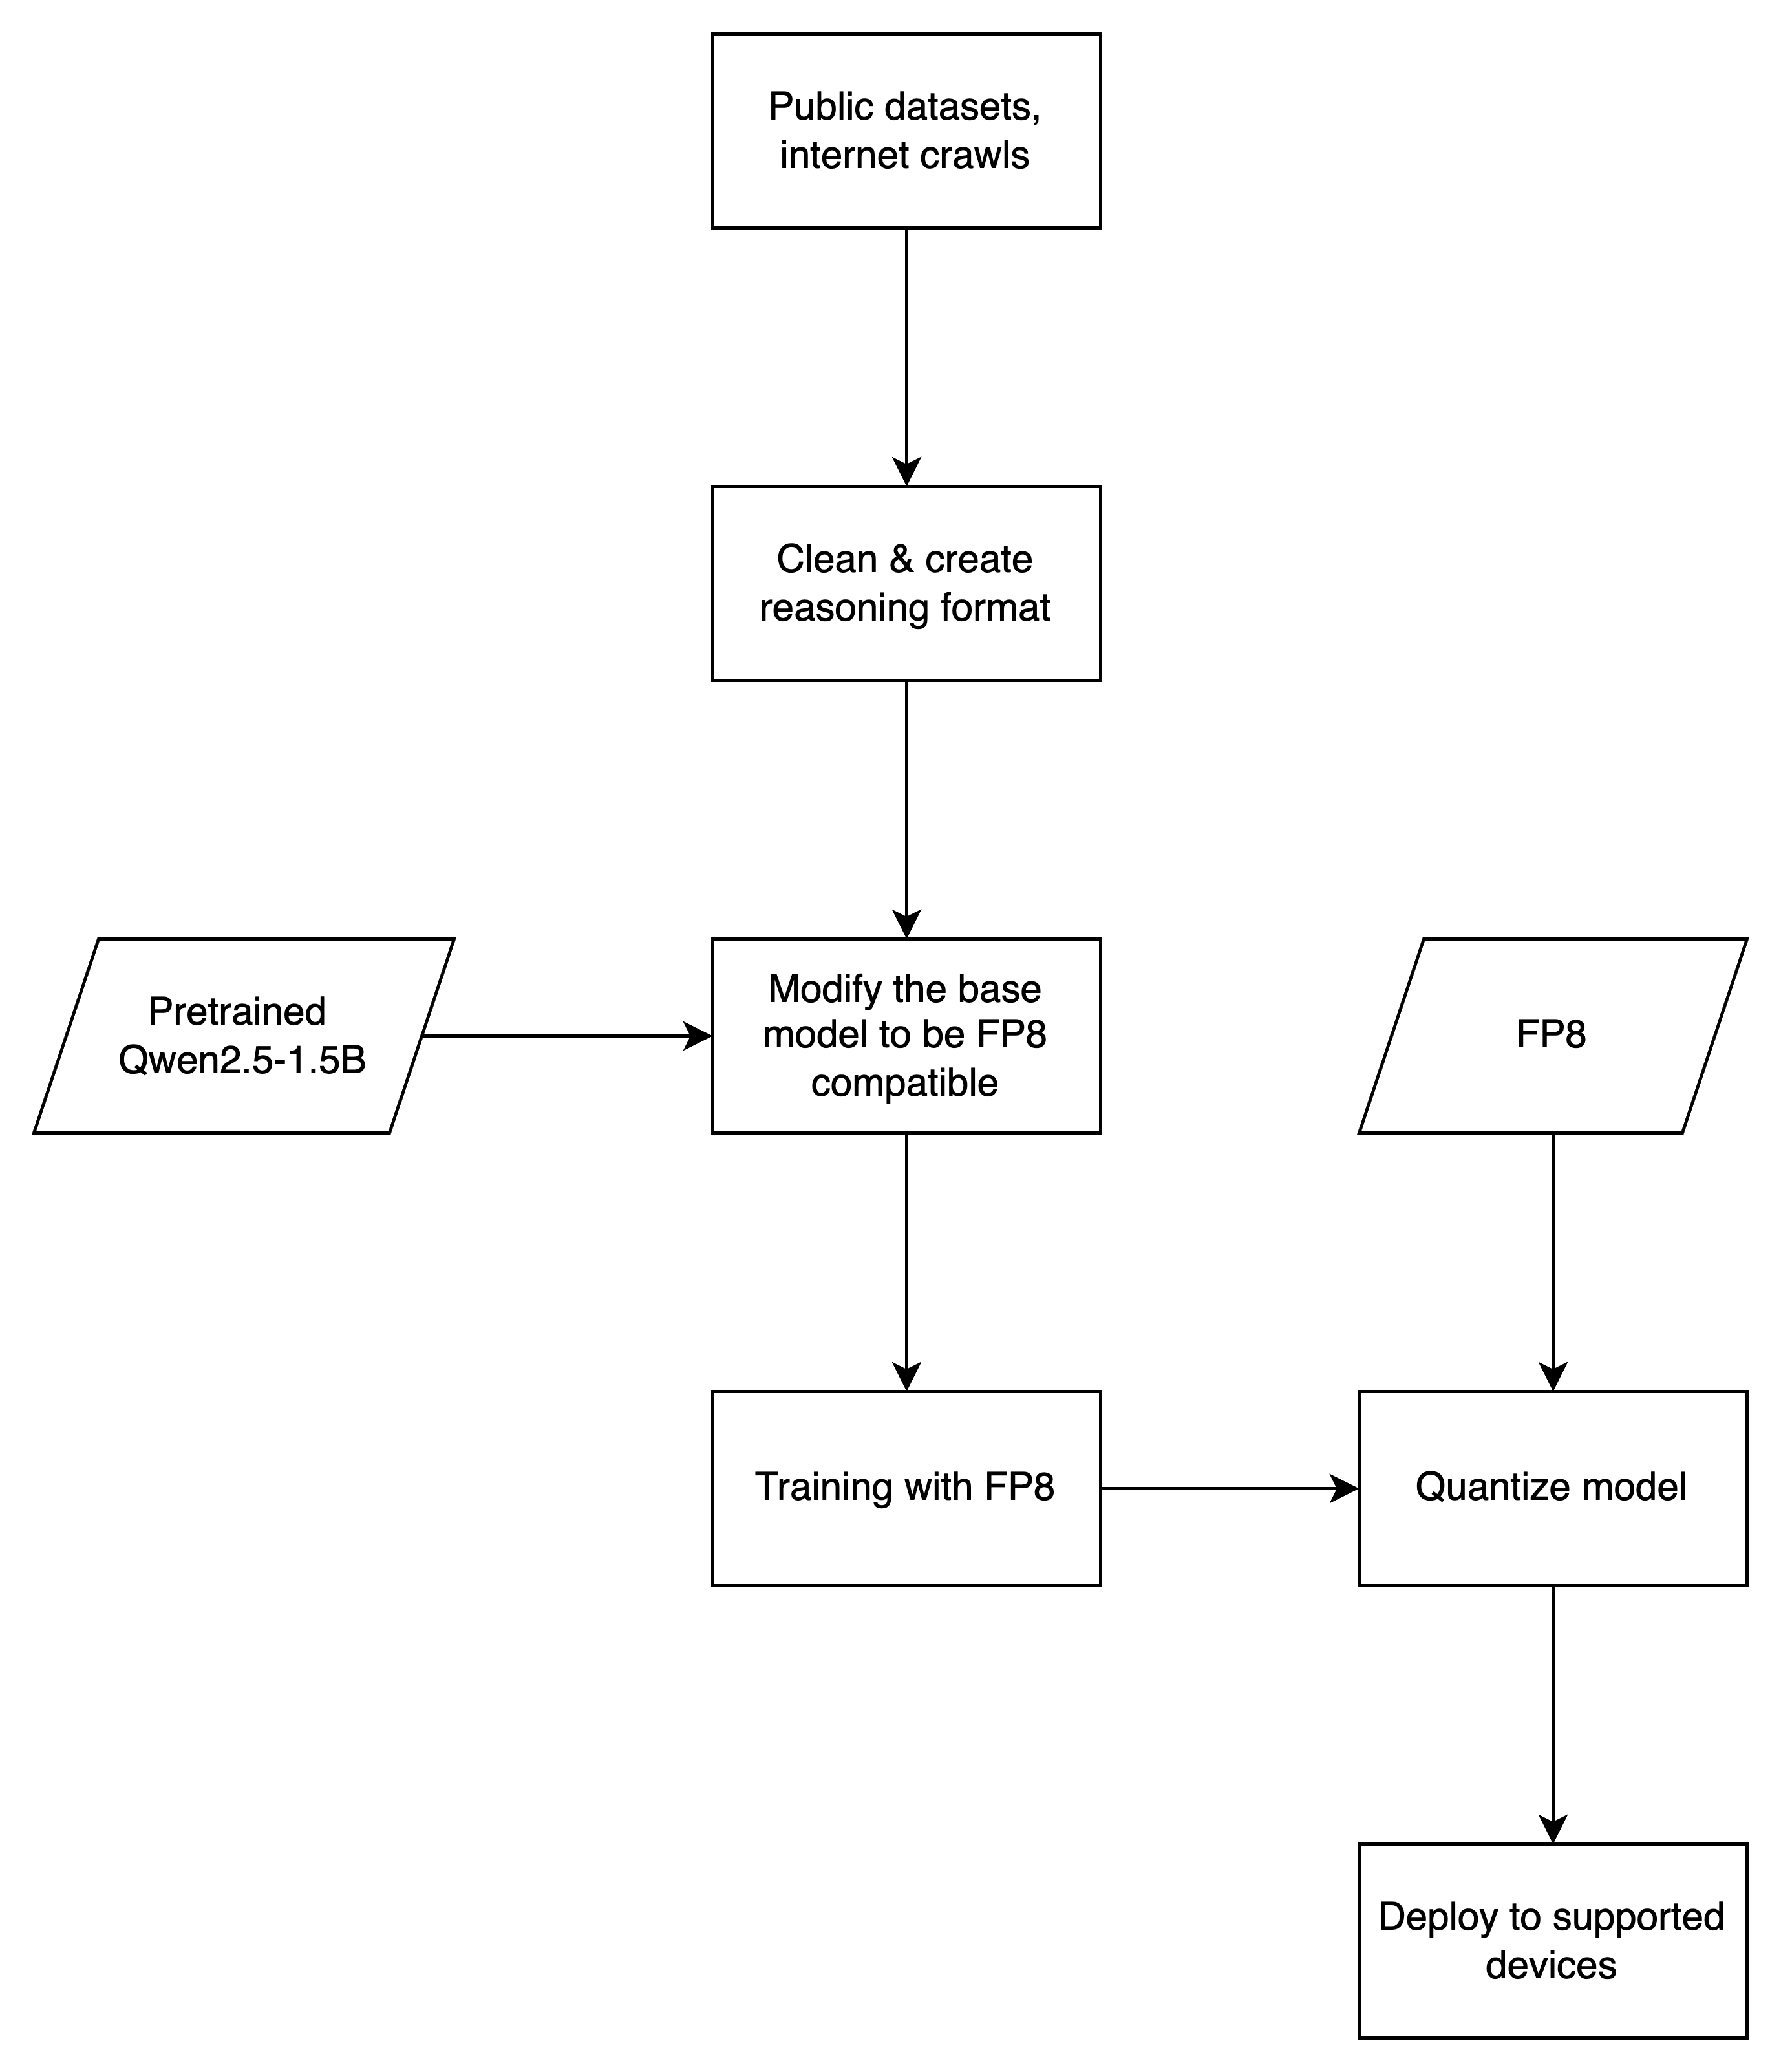
\includegraphics[width=0.75\linewidth]{figures/c1/overview.drawio.png}
    \caption{End-to-end pipeline for data construction, precision convert, fine-tune, and deploy the \textsc{Qwen2.5-1.5B} model.}
    \label{fig:overview}
\end{figure}

% \input{chapters/c1/c1_application}
